\documentclass{article}
\usepackage[utf8]{inputenc}
\usepackage{graphicx}
\usepackage{float}
\usepackage{ragged2e}
\usepackage{listings}
\usepackage{whilecode2}
\usepackage{verbatim}

\title{Practica 4}
\author{Enrique Narbona Luque}
\date{December 2022}

\begin{document}

\maketitle\LARGE{\underline{Activities}}

\vspace{4mm}

\RaggedRight{\section{\large{Create the simplest WHILE program that computes the diverge function(with zero arguments) and compute the codification of its code.}}}

\vspace{5mm}

\normalsize

La secuencia de instrucciones del programa sería la siguiente:

\vspace{3mm}

Q = (0,s)

s:

$ X1 \Assig X1 + 1 $

$ while X1 \not = 0 do $

$ X1 \Assig X1 $

od

\vspace{5mm}

Haciendo los cálculos tenemos:

\vspace{2mm}

$codi(S1) = 2$

$codi(S2) = 1$

$Codi(S21) = god (codi(S21)) - 1 = god(1) - 1 = 3 - 1 = 2$

$codi(s2) = 5\sigma21(1-1,Codi(S21)) + 4 = 5 5\sigma21(0,2) + 4 = 29$

$Codi(S) = god(codi(S1),codi(S2)) - 1 = god(2,29) - 1 = 139126$

\newpage

\large{\section{Create an Octave script that enumerates all the vectors.}}

 \vspace{5mm}

\RaggedRight{Sabemos que podemos establecer una biyección entre todos los vectores y N, solo necesitamos un código con un bucle que pueda imprimir todo el conjunto de los vectores. El siguiente código imprime los N primeros vectores:}

\vspace{5mm}

% Set the dimensions of the vectors

n = 3; % number of dimensions

m = 2; % number of vectors

% Initialize an array to store the vectors

vectors = zeros(n, m);

% Enumerate all the vectors

for i = 1:m

  for j = 1:n
  
    vectors(j, i) = i * j; % assign a value to each 
    
    % element of the vector
    
  end
end


% Print the vectors

disp(vectors)

\vspace{5mm}

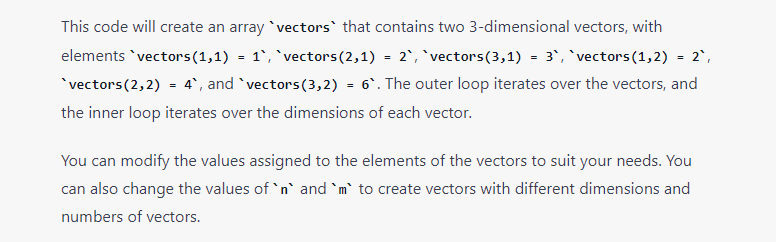
\includegraphics[scale=0.75]{4.2 TALF.png}

\newpage

\section{\large{Create an Octave script that enumerates all the WHILE programs.}}

\vspace{3mm}

Este caso se parece mucho al de la actividad 2, solo que se establece una biyección entre los programas WHILE y N, el código quedaría de la siguiente forma:

\vspace{4mm}

% Set the initial value of a counter variable

i = 0;

% Define the condition for the while loop

while (true)
  % Print the value of the counter variable
  
  N2WHILE(i)
  
  % Increment the counter variable
  
  i++;

end

\vspace{5mm}

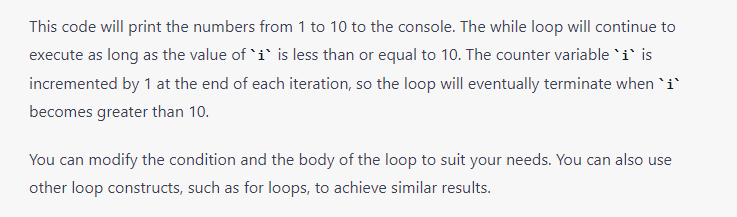
\includegraphics[scale=0.75]{4.3.png}

\newpage

\begin{verbatim}

  >> enumeracionWhile

  i = 0
  ans = (0, X_1 = 0)
  ans = 0
  i = 1
  ans = (1, X_1 = 0)
  ans = 1
  i = 2
  ans = (0, X_1 = 0; X_1 = 0)
  ans = 2
  i = 3
  ans = (2, X_1 = 0)
  ans = 3
  i = 4
  ans = (1, X_1 = 0; X_1 = 1)
  ans = 4
  i = 5
  ans = (0, X_1 = X_1)
  ans = 5
  i = 6
  ans = (3, X_1 = 0)
  ans = 6
  i = 7
  ans = (2, X_1 = 0; X_1 = 0)
  ans = 7
  i = 8
  ans = (1, X_1 = X_1)
  ans = 8
  i = 9
  ans = (1, X_1 = 0; X_1 = 1; X_1 = 0)
  ans = 9
  i = 10
  ans = (4, X_1 = 0)
  ans = 10
  i = 11
  ans = (3, X_1 = 0; X_1 = 0)
  ans = 11
  i = 12
  ans = (2, X_1 = X_1)
  ans = 12
  i = 13
  ans = (1, X_1 = 0; X_1 = 0; X_1 = 0)
  ans = 13
  i = 14
  ans = (0, X_1 = X_1; X_1 = 0)
  ans = 14
  i = 15
\end{verbatim}

\end{document}
